\section{High-dimensional Local Data Analysis in Locally Optimized Projections}
As described in the workflow, the proposed method supports a four-step exploration. In this section, we'll elaborate details of our method in each step of the exploration process.
\label{section:method}
\subsection{Discovering Interesting Local Focus}
Following Shneiderman's suggestion~\cite{DBLP:conf/vl/Shneiderman96}, we first provide the PCA projection as an overview of the data. Then we help the user find an interesting subset as the focus of subsequent local analysis.

In a projection, there are two situations where some local data is considered interesting. The first case is about distance distortion. Incorrect distances result in false neighborhoods. Closely distributed data may be far away in the original space and vice versa. Data involved in a distorted local area is regarded informative in the projection. It's also the basic idea in previous works concerning about data locality~\cite{DBLP:journals/cg/MartinsCMT14}~\cite{DBLP:journals/tvcg/StahnkeDMT16}. But such analysis only focuses on each datum at a time. It's hard to describe a group of data in this context. That's why we consider the second type, where the data is involved in some featured relationships, like being an outlier or a cluster. The relationship may have been weakened (e.g. a false cluster), but it's still strong enough to appear in the current projection. Hence, it makes a reasonable focus for a further study. Besides, it's suitable to describe a group of data in the context of relationships, rather than distance errors.

To put it simply, distortion analysis focuses more on the neighborhood of a single datum. Relationship analysis promotes the study of a data group. Regarding the two cases, we adopt different means to help the user find an interesting local focus.

\begin{figure}[htbp]
\centering
\subfigure[Datum Suggestion]{
	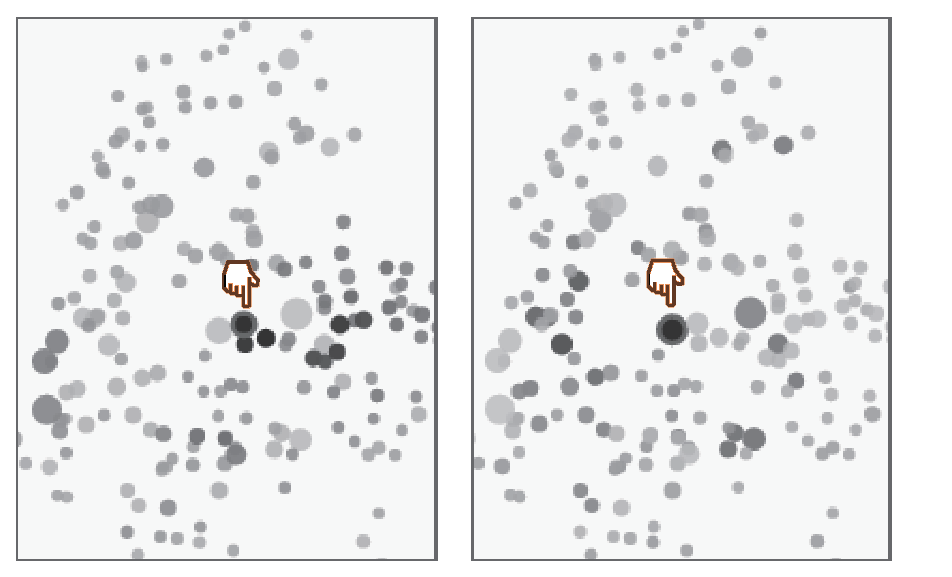
\includegraphics[width=0.48\linewidth]{images/suggestion_point.eps}
}
\subfigure[Cluster Suggestion]{
	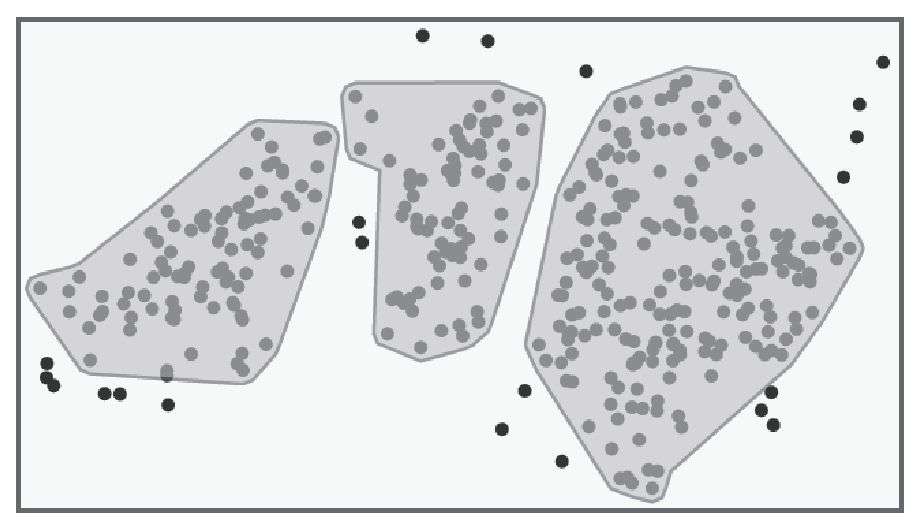
\includegraphics[width=0.46\linewidth]{images/suggestion_group.eps}
}
  \caption{Focus Suggestions}
\label{fig:suggestions}
  \end{figure}

\subsubsection{Datum Suggestion Based on Distance Distortion}
For any given projection, we consider a datum interesting if its distances to other data have been severely distorted. To measure the distortion, we accumulate distance errors for each datum in the projection:
\begin{equation}
Error(\mathbf{x}_{i}^{\prime}) = \sum\limits_{j=1}^{n}(Dist(\mathbf{x}_{i}, \mathbf{x}_{j}) - Dist(\mathbf{x}_{i}^{\prime}, \mathbf{x}_{j}^{\prime}))^{2}, i = 1,2,\cdots n
\end{equation}
Here the $\mathbf{x}_{i}$ and $\mathbf{x}_{i}^{\prime}$ represents the original data and the projected data respectively. Distance is measured by the Euclidean distance metric, taking into account all dimensions. We use point size to encode the accumulated distortion of each datum, as shown in Figure~\ref{fig:suggestions}(a).

On the other hand, we provide interactive hints to reveal the real distances. The approach is similar to that used in~\cite{DBLP:journals/tvcg/StahnkeDMT16}, but uses a different metaphor. When user hovers on the projection, we construct a so-called 'high-dimensional lantern' using interpolation. Assume that the hovered position corresponds to a two-dimensional datum $\mathbf{p}^{\prime}$, we interpolate its high-dimensional counterpart as follows:
\begin{equation}
\mathbf{p} = \sum\limits_{i=1}^{n}\mathbf{w}_{i}\cdot\mathbf{x}_{i} =  \sum\limits_{i=1}^{n} \left (\frac{Dist(\mathbf{x}_{i}^{\prime}, \mathbf{p}^{\prime})^{-1}}{\sum\limits_{j=1}^{n}Dist(\mathbf{x}_{j}^{\prime}, \mathbf{p}^{\prime})^{-1}}\right )\cdot\mathbf{x}_{i}
\end{equation}
The interpolation weight $\mathbf{w}_{i}$ of data $\mathbf{x}_{i}$ depends on its distance to the hovered spot in the projection. Closer data get larger weights. When user hovers right on $\mathbf{x}_{i}^{\prime}$, $\mathbf{w}_{i}$ equals $1$ while all the other weights get $0$. The result equals to the original data: $\mathbf{p} = \mathbf{x}_{i}$.

By the interpolation, we aims to infer what kind of data is desired by the user. Then this desired point acts as a high-dimensional lantern, shedding lights on all the other data to indicate it distances to them. With the lighting metaphor, we encode distance information using the saturation tunnel in HSL color space:
\begin{equation}
\begin{split}
Saturation(\mathbf{x}_{i}^{\prime}) &= \max{\{(\alpha D_{i}^{2} + \beta D_{i} + \gamma)^{-1}, 1\}},\\
D_{i} &= Dist(\mathbf{x}_{i}, \mathbf{p}), \quad i = 1,2,\cdots n
\end{split}
\end{equation}
The data gets high saturation, if it's close to the interpolated point in the original space. The parameters $\alpha,\ \beta$ and $\gamma$ come from the inverse-square law of the lighting model. Empirical values are chosen to accommodate most datasets. Users can hover on any datum to check its neighborhood. If the neighborhood has been distorted, its lights will not be able to illuminate its neighbors in the projection. In contrast, the real neighbors will appear in far away places. Figure~\ref{fig:suggestions}(a) demonstrates a case, where two neighboring points cannot affect each other. They are probably false neighbors due to distortion.

In summary, large data points are potentially interesting data with high distortion and inconsistent illumination. With the hints, user hovers around the projection like experiencing an adventure. He holds a lantern to explore unknown structures in the complex data space. Compared to~\cite{DBLP:journals/tvcg/StahnkeDMT16}, this method enables a more smooth and natural perception of distance information.

\subsubsection{Cluster Suggestion Based on Projected Relationships}
Automatic clustering algorithms play an important role in previous works~\cite{DBLP:conf/ieeevast/NamHMZI07}~\cite{DBLP:journals/cgf/LeeKCSP12}~\cite{DBLP:journals/cgf/LiuWTBP15}. Users are either given the clustering results, or assisted in tuning parameters of the algorithm. However, it's not intuitive to drive the clustering by parameters, since the algorithm is often a black box to users. Besides, it's hard for users to understand causes and details about the clusters, let alone modifying them or discovering new ones.

In our method, we decide not to provide global clustering results. Instead, we suggest an interesting group of data by examining projection clusters. It is based on the fact that, no additional or prior knowledge should be assumed in a free exploration. Users choose their focuses based on what they perceive. We only reveal real structures of the chosen focus. Users can still take full control of the clustering process, after they get the local insights.

Lots of clustering algorithms can be applied to identify projection clusters~\cite{DBLP:conf/ieeevast/Kandogan12}. We adopt a variant of DBSCAN~\cite{zhou2012research} whose parameters are adaptive to the data. We choose DBSCAN because it can efficiently identify clusters in any shape. The self-adaptive parameters make it applicable to most datasets without the need of manual tuning. Refer to Figure~\ref{fig:suggestions}(b) for the effect of cluster suggestion. The potential clusters are shown as contours. Users can choose any suggested cluster by simply clicking on it. To be clear, the suggestion only clarifies dominant relationships perceived by the user. It doesn't provide any extra information beyond the projection. If the user doesn't feel satisfied with the suggestion, he can choose his own focus by brushing the data.

\subsection{Featured Projections of the Focus}
We call a chosen datum the focus point, and call a chosen group the focus group. After some focus is chosen, we generate projections to either reduce its distortion, or enhance its local relationships.

\subsubsection{Distortion Reduced Projection}
For a focus point, we seek a projection to reduce its accumulated distance distortions. Let $\mathbf{P}$ be the focus point, we aim to solve the following optimization problem:
\begin{equation}
\min Error(\mathbf{P}) = \min_{\mathbf{A}}  \sum\limits_{i=1}^{n}(Dist(\mathbf{P}, \mathbf{x}_{i}) - Dist(\mathbf{PA}, \mathbf{x}_{i}^{\prime}))^{2}
\end{equation}
Here the term $\mathbf{A}$ represents the projection matrix. The projected focus point is $\mathbf{P^{\prime}} = \mathbf{PA}$. It can be proved that (refer to the appendix), the problem is equivalent to the following form:
\begin{equation}
\label{equation:center-shiftedPCA}
\max_{\mathbf{A}}  \sum\limits_{i=1}^{n}Dist(\mathbf{PA}, \mathbf{x}_{i}^{\prime})^{2}
\end{equation}
Note that if we replace $\mathbf{P}$ with the center of data $\mathbf{\bar{x}}$, the optimization will directly lead to PCA projection. In other words, the optimization can be regarded as PCA with a shifted center (i.e. the chosen focus). This center can reach its lowest distortion level. In turn, PCA can be thought of a single-datum distortion reduction. It lowers the overall distortion level, by helping the average datum. Figure~\ref{fig:car}(c) demonstrates the actual effect of our center-shifted PCA. As a result, the other data have more accurate distances towards the focus. False neighbors will be pulled away, leaving a more authentic neighborhood around the focus. Compared to the simple distance correction used in~\cite{DBLP:journals/tvcg/StahnkeDMT16}, our method preserves all benefits of a linear projection, rather than mere point-wise distances. It provides rich dimensional context, and help maintain a consistent mental model of the data space. In Section~\ref{subsubsection:relationship_enhancement}, we will further interpret this projection in the context of data relationships.

\subsubsection{Featured Local Relationships}
For a focus group, we first examine what kinds of relationships are of interest in the local analysis. Since relationships are defined based on distances, we can take a look at the distance matrix. Given the group, the distance matrix of all data is divided into three parts (Figure~\ref{fig:local_relationships}(a)). The first part describes distances between group members. The second part is about distances between the group and the other data. The last part describes distances among the context data. Since the last part has nothing to do with the focus, we simply ignore it. For the remaining parts, we consider the chosen data to be either 'similar' or 'dissimilar'.

\begin{figure}[htbp]
\centering
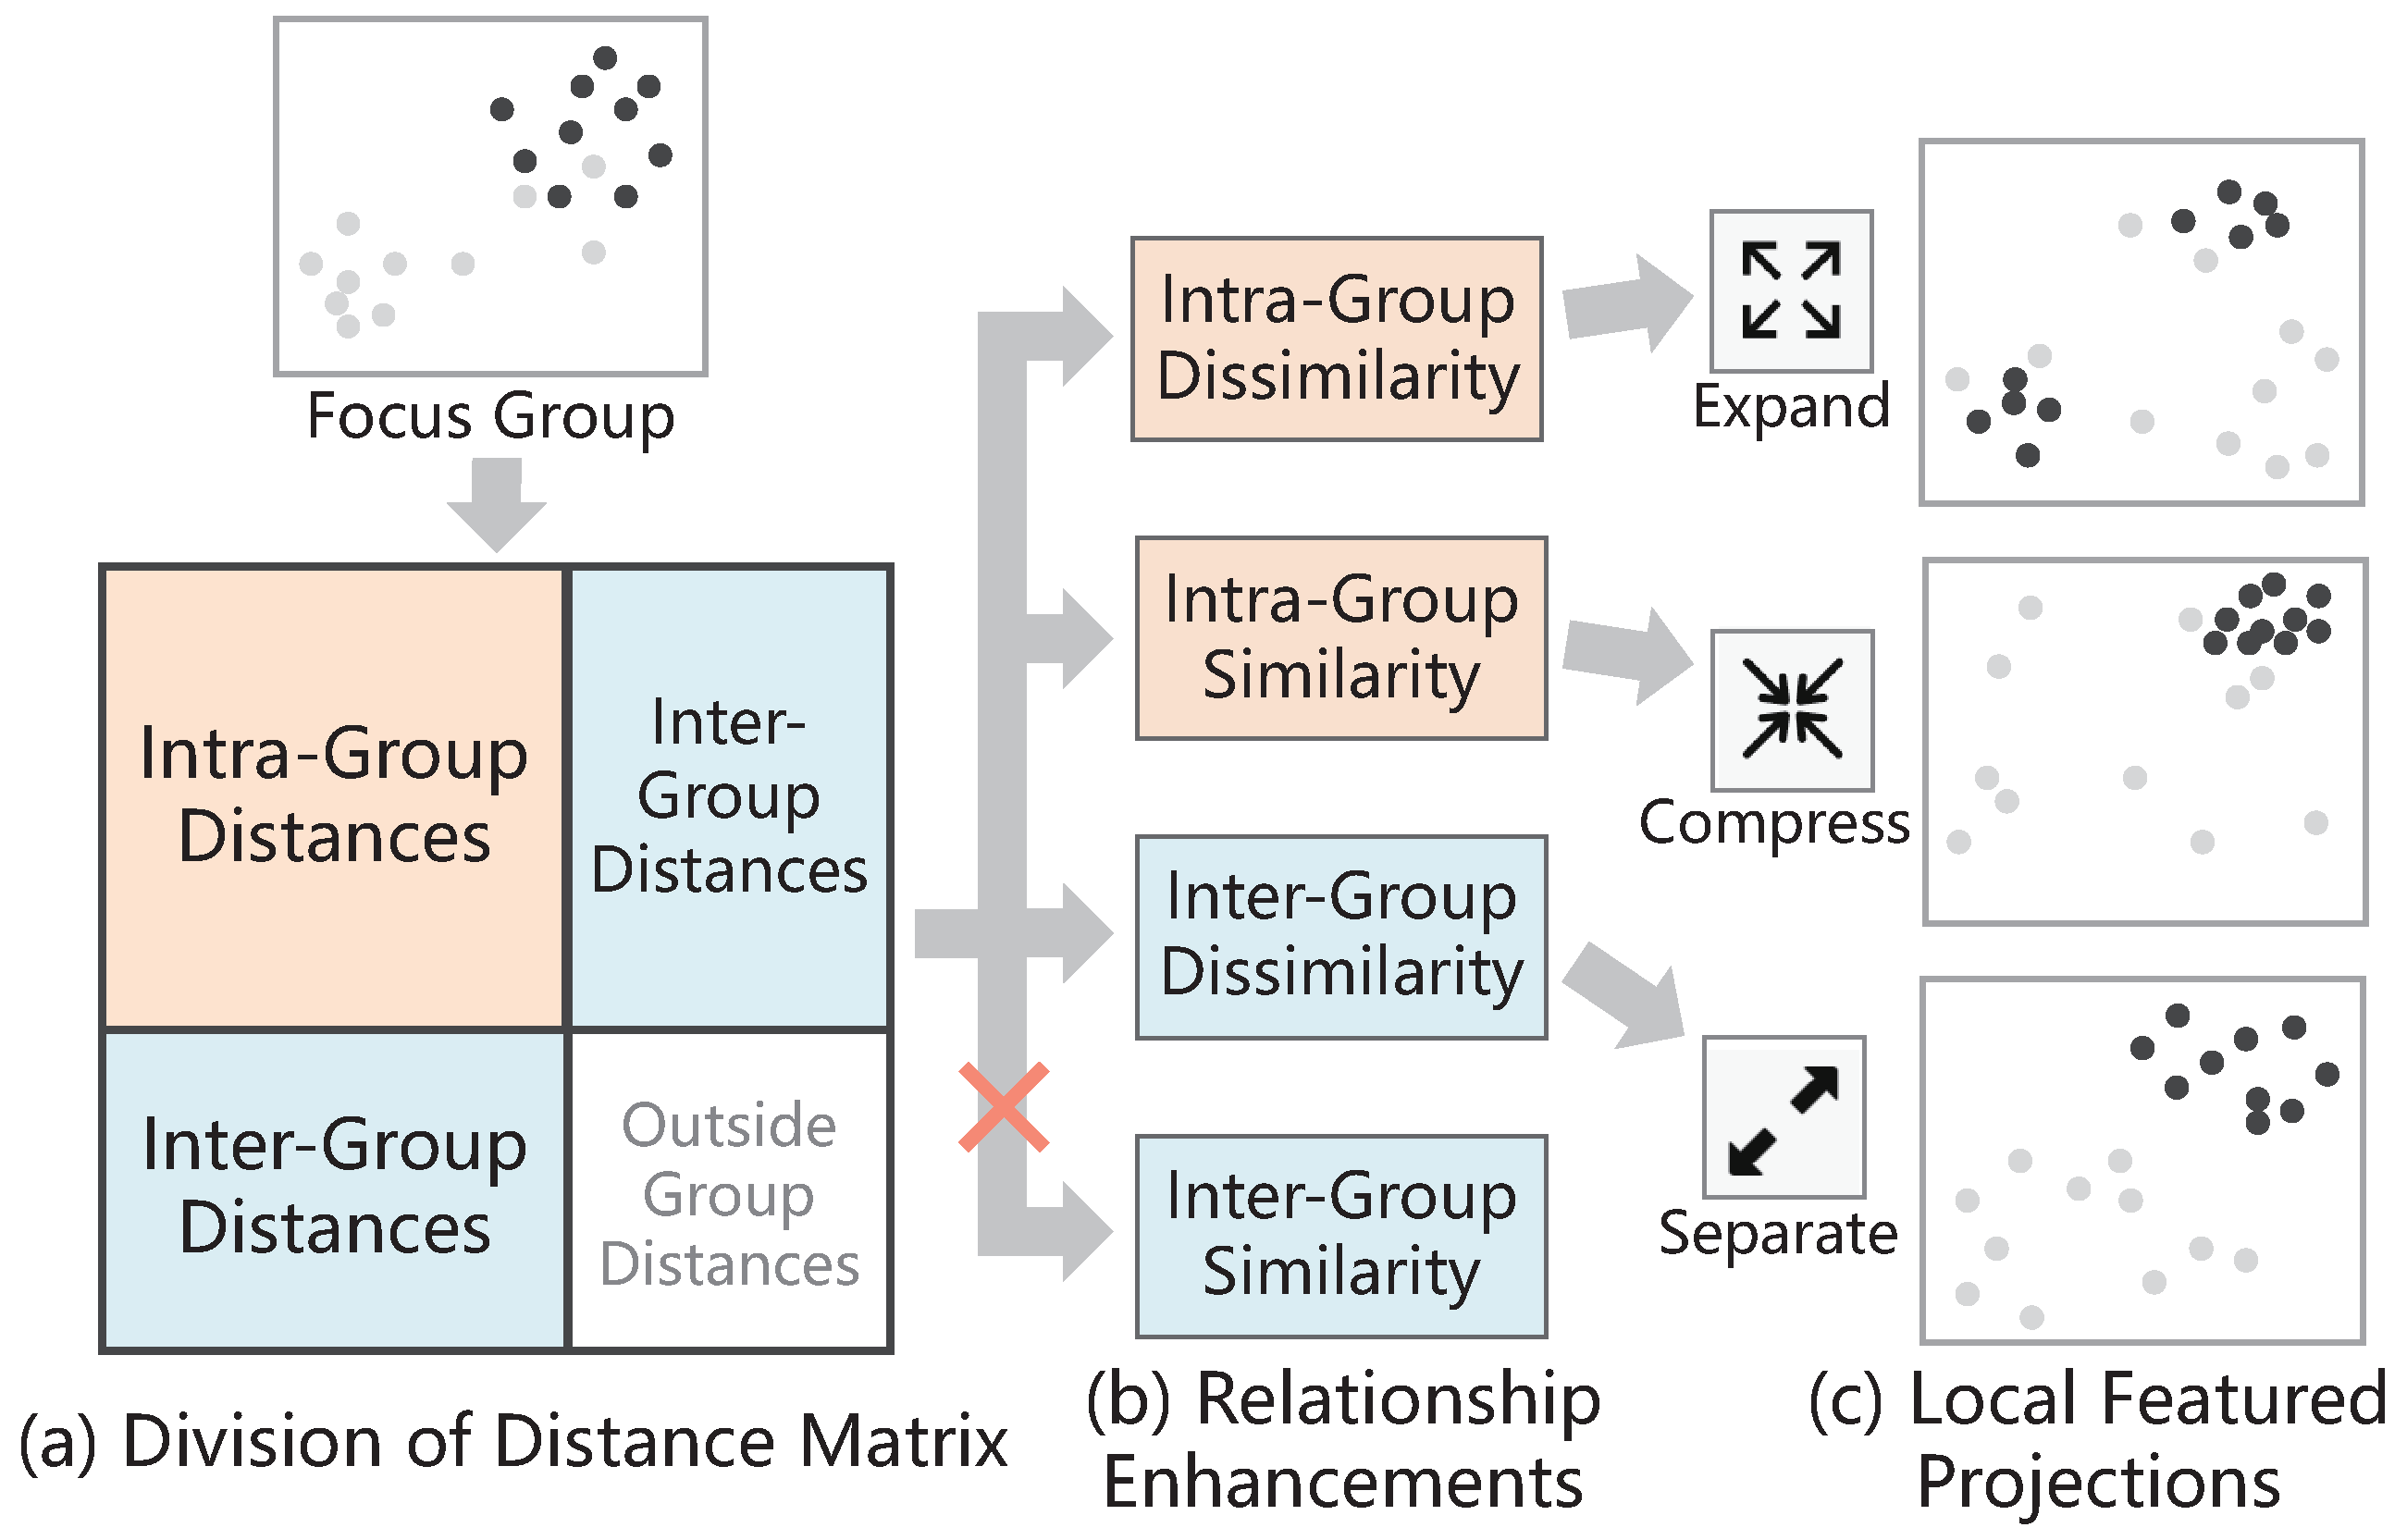
\includegraphics[width=1\linewidth]{images/enhancement1.eps}
  \caption{Enhancing featured local relationships}
\label{fig:local_relationships}
  \end{figure}

By revealing the similarities among group members, we show users in which aspects the data are most similar. It helps to comprehend why these data gather into a cluster in the projection. Enhancing dissimilarities, on the other hand, tells about the major differences among group members. Moreover, if there are sub-clusters within the group, the differences among them will be more prominent. This can reveal hidden local relationships.  Similarities between the group and the others is not of interest, as far as we are concerned. In contrast, by enhancing the dissimilarities, we can show why the focus group is different from the others. The idea resembles that of Linear Discriminant Analysis (LDA), expect that we did not regard the other data as a same class. In summary, three types of relationships are found most informative in the local analysis. We call them intra-group similarity, intra-group dissimilarity and inter-group dissimilarity respectively (Figure~\ref{fig:local_relationships}(b)).

\subsubsection{Relationship Enhanced Projections}
\label{subsubsection:relationship_enhancement}
With the three types of relationships, we first translate them in the context of data distances. Then we adopt projection pursuit to find linear projections for the enhancement.

Enhancing similarities or dissimilarities, equals to decreasing or enlarging data distances in the projection. For a focus group $G$, we enhance the intra-group dissimilarities by:
\begin{equation}
\max \sum\limits_{\mathbf{x}_{i}^{\prime}, \mathbf{x}_{j}^{\prime} \in G} Dist(\mathbf{x}_{i}^{\prime}, \mathbf{x}_{j}^{\prime})^{2} = \max_{\mathbf{A}} \sum\limits_{\mathbf{x}_{i}, \mathbf{x}_{j} \in G} Dist(\mathbf{x}_{i}\mathbf{A}, \mathbf{x}_{j}\mathbf{A})^{2}
\end{equation}
For simplicity, we call this optimization the \textbf{Expand} metric, since the focus group will be expanded in the resulting projection. The metric actually leads to a local PCA projection. Likewise, we enhance the similarities by maximizing the same metric:
\begin{equation}
\max_{\mathbf{A}} \sum\limits_{\mathbf{x}_{i}, \mathbf{x}_{j} \in G} Dist(\mathbf{x}_{i}\mathbf{A}, \mathbf{x}_{j}\mathbf{A})^{2}
\end{equation}
We call it the \textbf{Compress} metric, as the opposite of Expand. At last, we enhance the inter-focus dissimilarities by enlarging distances between the group and the other data:
\begin{equation}
\label{equation:Separate}
\max_{\mathbf{A}} \sum\limits_{\mathbf{x}_{i} \in G} \sum\limits_{\mathbf{x}_{j} \in \bar{G}} Dist(\mathbf{x}_{i}\mathbf{A}, \mathbf{x}_{j}\mathbf{A})^{2}
\end{equation}
This one is called the \textbf{Separate} metric. Figure~\ref{fig:local_relationships}(c) illustrate projections of all three metrics.

In fact, we can see a focus point as a group containing only one datum. There will not be Compress or Expand projections without multiple group members. But the Separate metric simply degrades to the single-datum distortion reduction (compare equation~(\ref{equation:center-shiftedPCA}) and~(\ref{equation:Separate})). That is, a datum has the lowest distortions, when it's far away from the others in the projection. This enables us to combine all featured projections into the same framework.

\subsubsection{Subspace Suggestion}
All dimensions are considered when pursuing the featured projections. However, only a few of them truly contribute to the features. The redundant dimensions will interfere with the analysis. That's why we need to reveal a subspace where features are most prominent.

In a sense, projection pursuit is a process to identify the most featured dimensions. We can make reliable suggestions according to its results. To be specific, we choose a subspace based on the projection found in the original space. Then in the chosen subspace, we do optimizations again to get the final results.

Given a projection, we first calculate the weight of each dimension:
\begin{equation}
W(d_{i}) = \left \|  \mathbf{a}_{i}\right \|_{2}, i = 1,2,\cdots m
\end{equation}
Here, $\mathbf{a}_{i}$ is the projected unit vector of dimension $d_{i}$. Its squared length acts as the weight. Then we rank all dimensions according to their weights: $W(d_{1}^{*}) > W(d_{2}^{*}) > \cdots >W(d_{m}^{*})$. All weights sum to 1. We pick out those with large weights, until their sum exceeds a certain threshold:
\begin{equation}
\begin{split}
&Subspace = \{d_{i}^{*}| i = 1,2, \cdots L \},\\
&s.t.\ \sum\limits_{j=1}^{L} W(d_{j}^{*}) \leq R \ \text{and}\ \sum\limits_{j=1}^{L+1} W(d_{j}^{*}) > R
\end{split}
\end{equation}
In fact, it is the same strategy as rank-by-feature~\cite{DBLP:journals/ivs/SeoS05}, except that our feature scores are dimension weights of a featured projection. The sum of weights is called the \textbf{subspace score}. It indicates how strong the chosen subspace is related to the features. The threshold $R$ is 0.75 by default, cutting down at least $25\%$ redundant dimensions. Users are informed of the weights at any time. They can change $R$ to include or exclude dimensions. After the subspace is chosen, we get the final result via a second-time projection pursuit in that subspace. The refined projection will be easier to interpret with only the most featured dimensions. But users can always decide whether to run the suggestion, or simply accept the original results.

\note{related to rank-by-feature}

\subsection{Modifying the Focus}
For a focus point, a distortion reduced projection is the final step. But for a focus group, it still needs to be modified. The featured projections support this task, by revealing the local insights.

The Expand projection shows minor relationships hidden in the group. Sub-clusters and outliers can be found. It helps to trim the focus into a more consistent cluster. The Compress projection not only shows similar aspects within the group. There could be other data who resemble the focus in these aspects. They will be drawn closer to the group in the projection, claiming to be potential members. The user may have missed them when making the selection. This projection can be used to regain the missing parts. The Separate projection exhibits differences between the group and the other data. If there are boundary points, they will stand out in the projection. It facilitate the study of cluster boundaries. The above benefits largely owe to the combination of local optimization and focus + context technique. In previous works with only local projections~\cite{DBLP:journals/tvcg/YuanRWG13}, it's hard to modify a focus without any context information.

We support the modification by providing two other brushing modes. In the 'Increase' mode, whatever chosen by the user will be added into the focus group. In the 'Decrease' mode, the user can choose among group members without being affected by the other data. After the modification is made, all featured projections will be updated. Smooth transitions are applied during the update. We keep an orthogonal mapping in each frame of the transition~\cite{cook2004computational}, in order to help maintain an intact mental model of the data space. The user can continue the analysis and modification, until he gets a satisfying result.

\subsection{Focus Comparison in the Projection Map}
During the exploration, there will be times when the user needs to store the result. For example, when sub-clusters are found, the large cluster should be stored before the exploration goes into details. Besides, it's necessary to compare different focuses regarding their features. For these purpose, we provide the focus list, along with a map of all featured projections.

In the focus list, users can store the current focus or retrieve it at any time. Each focus is represented as a node (see Figure. ). Its size denotes the data size. Users can name a focus, or assign it some color. Specially, there is a fixed node called 'All Data'. Applying Expand metric to it will get the global PCA projection.

For every focus in the list, its featured projections are shown as glyphs in the projection map. Different glyphs represent different types of projections, as shown in Figure. \col{(Figure to be added.)} Dimension weights are also displayed to help compare the projections. Clicking on a glyph can retrieve the focus and the corresponding projection. To quantify distances between any two projection, we refer to the manifold learning domain. It has been proved that any two 2D projections lie on the same manifold, which is called the Grassmann manifold. We measure projection distances by geodesic distances on the manifold~\cite{absil2004riemannian}. The map is constructed based on the distance matrix using MDS.

In the projection map, users can compare features of different focuses. For example, two focus groups may have the same reasons for the grouping (i.e. intra-group similarities), while having different inner-group diversities (see Figure.). \col{(Figure to be added.)} It helps to understand different local data in the context of featured dimensions. In addition, users can plan their own high-dimensional tours in this map. A similar idea has been proposed in the TripAdvisor~\cite{DBLP:journals/tvcg/NamM13}, as an extension of the Grand Tour~\cite{asimov1985grand}~\cite{cook1995grand}. But their projections are driven by dimensions without explicit semantics. In comparison, each spot in our map is tightly related to some local data and a certain relationship. It makes the tour more targeted and easier to interpret.